\chapter{The \acl{CMS} Experiment at the \acl{LHC}}
\label{sec:experiment}
\section{Introduction}
The \acf{LHC}~\cite{lhc_design_report} is a proton-proton ($\Pp\Pp$) accelerator
located at the CERN particle physics laboratory near Geneva, Switzerland. It has
been designed to carry out a broad program of physics research at a number of
specialised detectors. This section will give a very brief introduction to the
\ac{LHC} itself. The \acf{CMS} experiment, a large, general purpose detector at
the \ac{LHC}, will be discussed in detail.

\section{The \acl{LHC}}
The \ac{LHC} is a circular synchrotron, \unit{27}{\kilo\metre} in circumference,
sitting on the border between France and Switzerland. It has been built in a
tunnel initially constructed to house the \ac{LEP} accelerator, buried at a
depth of between 50 and \unit{175}{\metre} underground. Whilst primarily, a
$\Pp\Pp$ accelarator, the \ac{LHC} will also undertake a heavy-ion physics
program. At full design specifications, 2808 bunches of protons will circulate
around each direction of the ring, colliding at a centre-of-mass energy of
\unit{14}{\TeV}. It is designed to eventually reach a proton bunch spacing of
\unit{25}{\ns} and an instantaneous luminosity of
\unit{$10^{34}$}{\rpsquare{\centi\metre}\usk\reciprocal\second}.

There are four primary experiments at the LHC: \ac{ALICE}, \ac{ATLAS}, \ac{CMS}
and \ac{LHCb}. Each one is constructed around one of the four interaction points
and records the shower of particles produced from the colliding protons. ATLAS
and CMS are large, general purpose detectors designed to search for a variety of
\ac{NP} signatures as well as making higher precision measurements of \ac{SM}
parameters. \ac{ALICE} is designed to examine the products of heavy-ion
collisions (principally lead-lead - although a number of configurations are
possible) in order to explore the quark gluon plasma and related
physics. Finally, the \ac{LHCb} experiment is optimised for the study of B-meson
decays. These are important for the study of CP violation within the \ac{SM} but
might also provide potential avenues for the discovery of \ac{NP}.

In addition to the four larger detectors, two smaller experiments, \ac{LHCf} and
\ac{TOTEM} lie upstream of the \ac{ATLAS} and \ac{CMS} collision points in order
to probe more specialised forward physics phenomena.

\subsection{Accelerator Complex}
The \ac{LHC} ring itself is the final stage in an injector chain utilising a
series of accelerators built at CERN over the last 50 years. Each stage supplies
an incremental increase in the proton (or heavy ion) bunch energy. The first
stage in this chain is a linear accelerator, either the Linac2 for proton
injection or Linac3 during heavy-ion runs. The Linac2 injects protons into the
\ac{PSB} at an energy of \unit{50}{\mega\electronvolt}. Similarly, the ions
proceed first from the Linac3 to the \ac{LEIR} before finally arriving at the
\ac{PS}. From here on, the paths of the protons and heavy-ions are the
same. Proton bunches pass from the \ac{PSB} to the \ac{PS} at an energy of
\unit{1.4}{\giga\electronvolt} and then on to the \ac{SPS} at an energy of
\unit{28}{\giga\electronvolt}. Protons then arrive at the \ac{SPS}, where they
circulate around a ring \unit{2}{\kilo\metre} in diameter, and increasing their
energy to \unit{450}{\giga\electronvolt}. From here, kicker magnets inject the
bunches into the \ac{LHC} itself, where the energy is finally increased to the
design specified \unit{7}{\TeV} per beam.
\begin{figure}
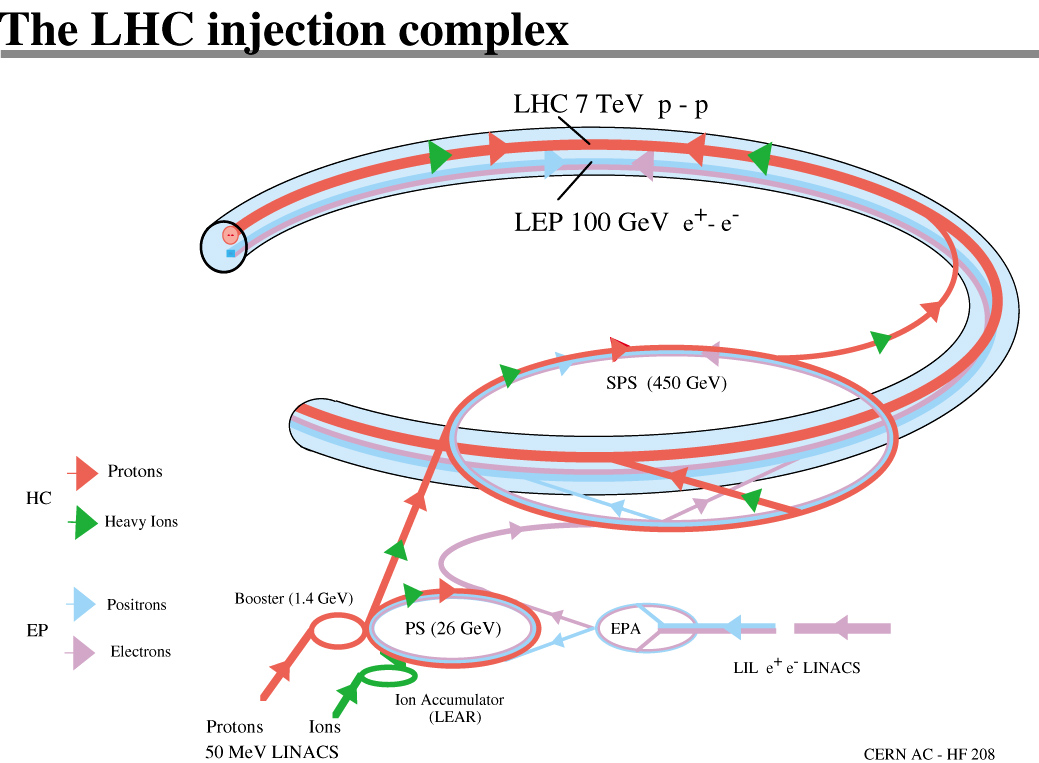
\includegraphics[width=0.9\textwidth]{fig/lhc-pho-1993-008}
\end{figure}

% TODO: More on the LHC beam etc.!

\ctable[
cap=LHC Accelerator Complex,
caption=LHC Accelerator Complex,
mincapwidth=0.5\textwidth,
pos=h
]{lcc}{
\tnote[a]{Heavy-Ions only}
}{\FL
Accelerator & Energy \ML
%
Linac2   & \unit{50}{\mega\electronvolt} \NN
Linac3\tmark[a]   & \unit{4.2}{\mega\electronvolt\per u} \ML
%
\acf{PSB} & \unit{1.4}{\giga\electronvolt} \NN
\acf{LEIR}\tmark[a]   & \unit{??}{\mega\electronvolt\per u} \ML
%
\acf{PS} & \unit{28}{\giga\electronvolt} \NN
\acf{SPS} & \unit{450}{\giga\electronvolt} \NN
\acf{LHC} & \unit{7}{\tera\electronvolt} \LL
}


\section{The \acl{CMS} Experiment}
\label{sec:cms}
\ac{CMS} is a large, general purpose detector~\cite{cms_jinst} at the
\ac{LHC}. It has been designed to search for the Higgs boson (see
Section~\ref{sec:sm_higgs}) as well as signatures of physics beyond the \ac{SM}.

The design goals of CMS were as follows (paraphrasing the technical proposal
document~\cite{cms_technical_proposal}):
\begin{enumerate}
\item a high quality, redundant muon system,
\item the best possible \ac{ECAL}
\item high quality central tracking to complement these two systems
\item an affordable detector
\end{enumerate}

\begin{figure}
\centering
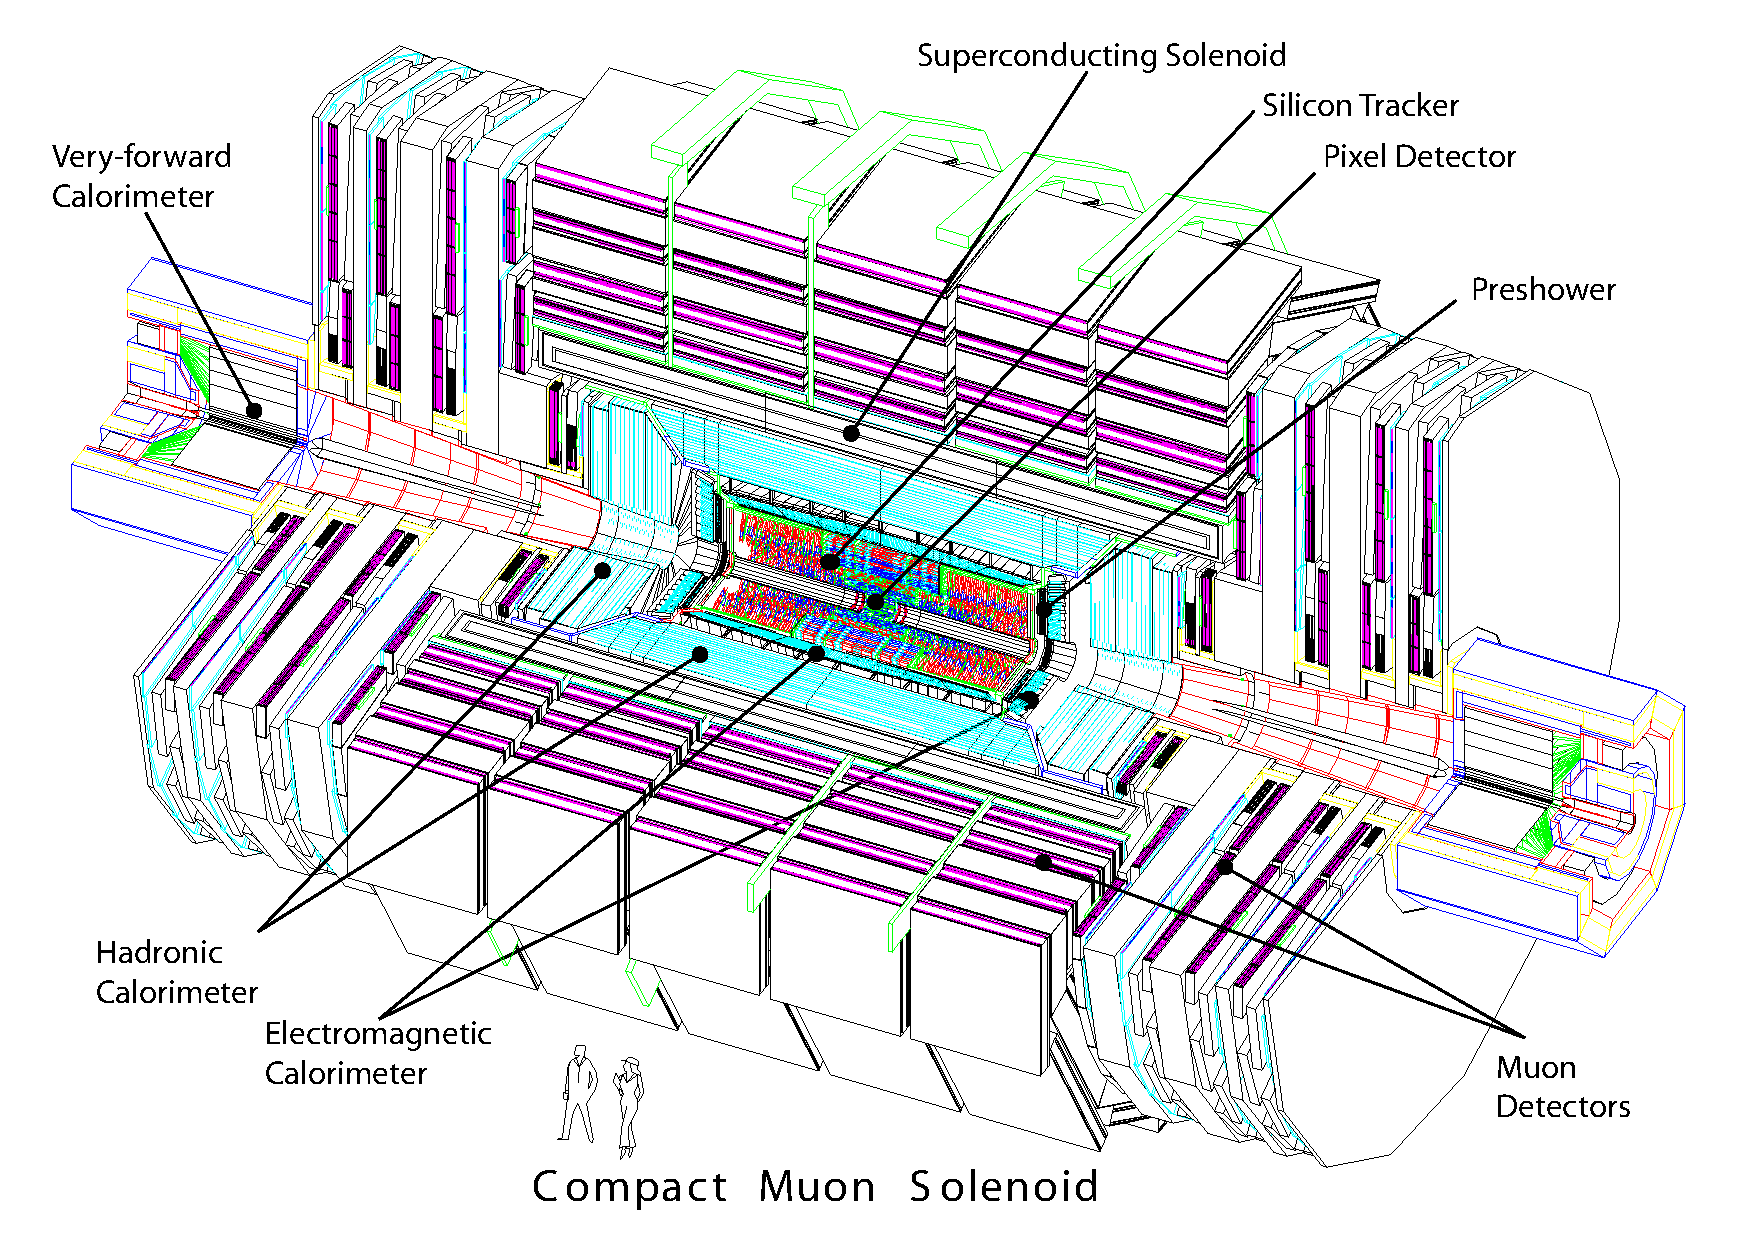
\includegraphics[width=0.7\textwidth]{fig/cms_complete_labelled}
\caption{The CMS Detector}
\label{fig:expt_cms}
\end{figure}

\ac{CMS} adopts a traditional cylindrical design (see
Figure~\ref{fig:expt_cms}), \unit{21.5}{\metre} in length and \unit{15}{\metre}
in diameter. A key feature of the detector is the \unit{4}{\tesla}
superconducting solenoid. The bending field supplied provides accurate muon
momentum resolution up to energies of \unit{$\approx$ 1}{\TeV}. The size of the
solenoid placed stringent limitations on the volume of the inner detector
subsystems (everything except for the muon chambers and return yoke).

\subsection{Coordinate System}
The coordinate system at \ac{CMS} is right-handed with its origin placed at the
nominal beam collision point inside \ac{CMS}. The $x$ axis is then defined to
point horizontally inwards towards the centre of the \ac{LHC} ring and the
$y$-axis vertically upwards. Therefore the $z$-axis is aligned along the
beam-line pointing towards the nearby Jura mountains. Often a cylindrical
coordinate system will be used with where the azimuthal angle, $\phi$, and
radial coordinate, $r$, span the $x-y$ plane. The azimuthal angle is measured
with respect to the $x$-axis. The pseudorapidity, $\eta = - \ln \tan
\frac{\theta}{2}$ where $\theta$ is the polar angle measured with respect to the
$z$-axis.

\subsection{Silicon Tracker}
The innermost subsystem of \ac{CMS} is the silicon tracker, designed to provide
highly precise measurements of particle trajectories close to the CMS
interaction point. It is shown in cross section in
Figure~\ref{fig:expt_tracker}. The tracker extends to pseudorapidities of
$|\eta|<2.5$ and has an active silicon area of more than
\unit{200}{\metre\squared}, making it the largest silicon tracker ever built.

\begin{figure}[h!]
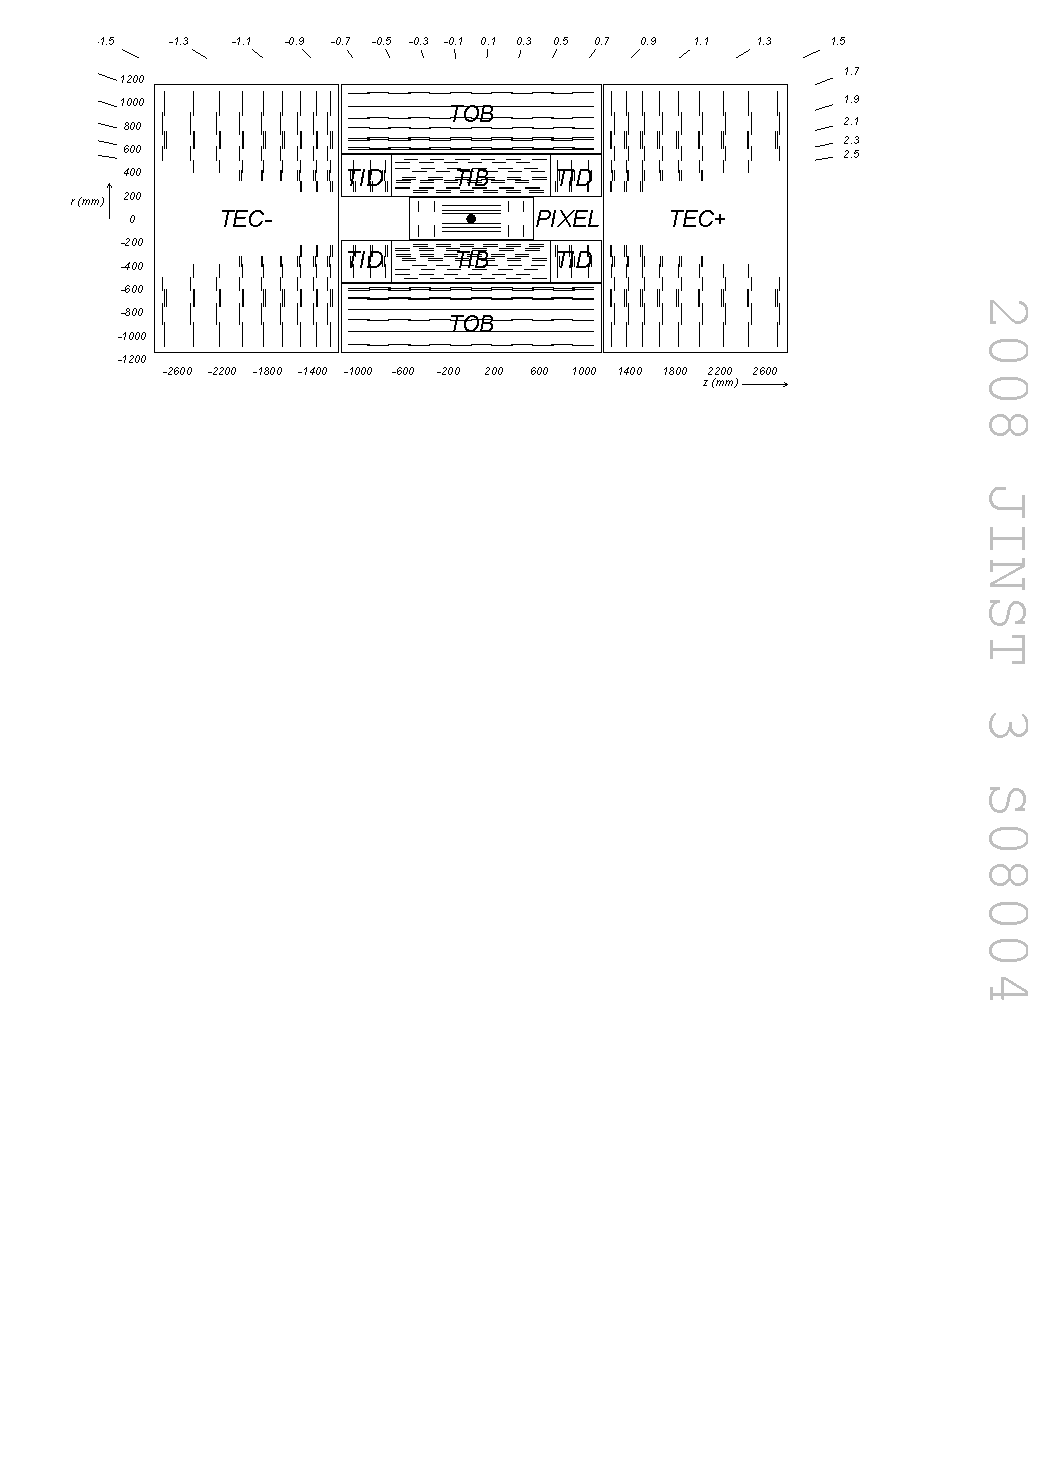
\includegraphics[width=\textwidth]{fig/tracker}
\caption{Schematic cross section through the CMS tracker. Each line represents a
  detector module. Double lines indicate back-to-back modules which deliver
  stereo hits~\cite{cms_jinst}.}
\label{fig:expt_tracker}
\end{figure}

The tracker design can be better understood by considering the expected particle
flux at design luminosity as a function of radial distance $r$ from the
beam-line.
\begin{itemize}
\item At $ r \approx \unit{10}{\cm}$ the particle flux is highest. Accordingly,
  the innermost layer of the CMS tracker is comprised of hybrid pixels. With an
  area of \unit{$100\times 150$}{\micro\metre\squared}, particle densities are
  $O(10^{-4})$ per pixel per LHC bunch crossing.
\item At a radius \unit{$20 < r < 55$}{\centi\metre}, reduced particle flux allows
  the use of silicon microstrip sensors. With a much larger area of
  $\unit{10}{\centi\metre}\times\unit{80}{\micro\metre}$, average particle
  densities are $O(10^{-2})$ per strip per bunch crossing.
\item At $ r > \unit{55}{\cm}$, still larger silicon strips can be used, with
  sizes up to $\unit{25}{\cm}\times\unit{180}{\micro\metre}$. This gives a
  particle density of $O(10^{-2})$ per strip per bunch crossing.
\end{itemize}

\subsubsection{Pixel Tracker}
The hybrid pixels are placed closest to the interaction point. As well as
maintaining an acceptable particle density per sensor, their close proximity to
the interaction point allows the origin of collision products to be accurately
determined. This is of particular importance for instance in B-tagging. In the
barrel region, 3 layers are placed at mean radii of 4.4, 7.3 and
\unit{10.2}{\cm}. The detector has a length of \unit{53}{\cm} in the $z$
direction. The end discs are instrumented with only two layers and are located
at $|z|=34.5, \unit{46.5}{\cm}$. The pixel modules in these layers are arranged
in a turbine-like layout.

\subsubsection{Strip Tracker}
Further from the interaction point, the tracker is instrumented with silicon
strip detectors. The barrel component can be further divided into the \ac{TIB}
and the \ac{TOB}. The \ac{TIB} is composed of 4 layers with the \ac{TOB}
comprising a further 6. The \ac{TOB} extends to $z = \pm
\unit{118}{\centi\metre}$. Beyond this are the endcaps which can again be split
into two components: the \ac{TEC} made up of 9 disks and the \ac{TID} 3. The
silicon micro strip sensors are \unit{320}{\micro\metre} thick and oriented
parallel to the $z$ axis in the barrel and radially in the disks.

Both the \ac{TIB} and \ac{TID} supply up to four measurements of $r\phi$. With a
strip-pitch of \unit{80}{\micro\metre} in the inner two layers and
\unit{120}{\micro\metre} in the outer two, the \ac{TIB} achieves a single point
resolution of \unit{23 and 35}{\micro\metre} respectively. In the \ac{TID}, the
strip pitch varies between \unit{100 and 141}{\micro\metre}.

The \ac{TOB} uses \unit{500}{\micro\metre} thick sensors with a strip-pitch of
\unit{183}{\micro\metre} in the first four layers and \unit{122}{\micro\metre} in
the outer two. This gives a single point resolution of \unit{53}{\micro\metre}
and \unit{35}{\micro\metre} respectively.

The first two layers of the \ac{TIB}, \ac{TOB} and \ac{TID} and rings 1, 2 and 5
of the \ac{TEC} are so-called stereo modules. These are double-sided modules
where the two layers of strips have a stereo angle of \unit{100}{\milli\radian}
between them. This provides additional resolution in the $z$ measurement in the
barrel (or $r$ in the endcaps). The resolution of this measurement is
\unit{230}{\micro\metre} and \unit{530}{\micro\metre} in the \ac{TIB} and
\ac{TOB} respectively.



\subsection{\acl{ECAL}}
The \ac{ECAL} surrounds the silicon tracker and provides a high resolution
measurement of electromagnetic showers within a homogeneous, hermetic
calorimeter~\cite{ecal_paper}. The barrel region along comprises 61,200 lead
tungstate (PbWO$_4$) crystals, with 7,324 in each of the two endcaps. This
material was chosen for its high density, short radiation length and small
Moli\`{e}re radius. Scintillation photons are then recorded by \ac{APD}s in the
barrel and \ac{VPT}s in the endcap. The driving motivation for the \ac{ECAL}
design was the detection of the low-mass favoured Higgs decay channel
$PH\longrightarrow\gamma\gamma$.

\subsubsection{\acl{EB}}
The \ac{EB} extends in rapidity to $|\eta|<1.479|$ with a crystal
segmentation of $360\times 85$ ($\eta-\phi$) in each half barrel. Each crystal
is slightly tapered with a cross-section of $0.0174\times0.0174$ in
$\eta-phi$. The crystals have a front cross section of \unit{$22\times
  22$}{\milli\metre\squared} and a length of \unit{230}{\milli\metre}
(corresponding to 25.8 radiation lengths).

\subsubsection{\acl{EE}}
The \ac{EE} occupies the rapidity range $1.479 < |\eta| < 3.0$. Crystals are
grouped into $5\times 5$ supercrystals within a carbon-fibre alveolar
structure. The endcaps are split into two halves, known as ``Dees'', each
holding 3,662 crystals.

The scintillation of the \ac{ECAL} crystals as well as the amplification of the
\acp{APD} varies as a function of temperature. This variation was found to be
\unit{$\approx 4\%$}{\per\celsius}. For this reason, the \ac{ECAL} temperature
is precisely regulated to within \unit{$\pm$ 0.05}{\celsius}.

\subsubsection{\ac{ECAL} Transparency and the \ac{CMS} Laser Monitoring System}
\label{sec:expt_laser_monitoring}
The PbWO$_4$ crystals that make up the \ac{ECAL} are radiation resistant but
quickly suffer a decrease in their optical transmission under
irradiation~\cite{ecal_transparency}. This is a result of the formation of
colour centres which absorb a fraction of the incident light. At a working
temperature of \unit{18}{\celsius}, the damage anneals leading to an equilibrium
in the optical transmission properties - constant with dose rate. The
consequence of this is a cyclic change in the optical transmission rate of the
crystals as the \ac{LHC} moves between colliding beams and machine
refills. Since this depends on dose rate, the effect is a function of \ac{LHC}
luminosity and rapidity. It is expected to range from a shift of $\sim 2\%$ in
the barrel at low luminosity to $> 10\%$ in the endcaps at high luminosity. The
magnitude of this effect on energy and momentum measurements would be disastrous
if not properly accounted for. Correction of the reconstruction necessitates
constant monitoring of the transparency - a task performed by the laser
monitoring subsystem~\cite{laser_monitoring}.

Three lasers are used for the transparency measurement: two blue ($\lambda
\approx \unit{440}{\nano\metre}$) and one near-infrared ($\lambda \approx
\unit{796}{\nano\metre}$). The blue laser (with a second fitted for redundancy
purposes) is close to the scintillation emission peak and thus can be used to
track the changes in the crystal transparency. The near-infrared laser is far
from the emission peak and thus relatively stable to changes in the
transparency. This can be used to verify the stability of the system. The lasers
are distributed to the crystals via optical fibres and a series of
fan-outs. Approximately 1\% of the \ac{LHC} beam gap of
\unit{3.17}{\micro\second} is used for transparency monitoring. A full scan of
the entire \ac{ECAL} can be achieved in approximately 30~minutes. The lasers can
be pulsed at $\approx \unit{80}{\mega\hertz}$ with a pulse timing jitter of
\unit{3}{\nano\second}. This is adequate for synchronisation with the \ac{LHC}
bunch crossings.

The transparency of the crystals is derived from the response of the \ac{APD}
normalised to the height of the laser pulse, as measured using a silicon
photodiode. Due to differences in path length and optical spectra between the
laser and the scintillation light, the transparency of the crystals may be
related to the measured transparency via a power law.

\subsection{\acl{HCAL}}
Accurate measurement of hadronic showers is crucial for analyses involving jets
or missing energy signatures. The \ac{HCAL}~\cite{hcal_paper} lies between the
outer edge of the ECAL and the inner edge of the solenoid ($\unit{1.77}{\metre}
< r < \unit{2.95}{\metre}$). This constrains the size of the \ac{HCAL} to a
relatively compact design and necessitates the placement of a ``tail catcher''
outside of the solenoid.

\subsubsection{\acl{HB}}
The \ac{HB} comprises 36 azimuthal wedges, with 18 in each half barrel. Each
wedge consists of alternating layers of brass absorber plates and plastic
scintillators. The light from these plates is then carried via
wavelength-shifting fibres to a \ac{HPD} for readout. The number of interaction
lengths increases with polar angle, from 5.82 at $90\degrees$ to 10.6 at
$|\eta|=1.3$~\cite{hcal_design}.

\subsubsection{\acl{HE}}
The \ac{HE} covers the rapidity range $1.3 < |\eta| < 3$ and receives a larger
radiation flux than the \ac{HB}. Each endcap consists of 36 wedges, and
wavelength shifting fibres are once again used to take like from plastic
scintillators to \acp{HPD}. Including the \ac{ECAL}, the \ac{HE} depth is
equivalent to $\approx 10$ interaction lengths.

\subsubsection{\acl{HO}}
The \ac{HO} or ``tail catcher'' provides increased sampling depth in the
rapidity region $|\eta| < 1.3$ where the \ac{HB} and \ac{EB} do not provide
sufficient containment. Since the \ac{HO} lies outside the solenoid, its design
is constrained by that of the muon chambers - with 5 rings in $\eta$. The
solenoid coil provides additional absorption, giving the calorimeter system a
minimum depth of 11.6 interaction lengths.

\subsubsection{\acl{HF}}
The \ac{HF} is positioned in the rapidity range $|\eta|>3$ and consequently must
endure a much larger particle flux - approximately \unit{760}{\GeV} per
proton-proton interaction (versus $\approx \unit{100}{\GeV}$ for the rest of the
detector). Radiation hardness was thus a leading consideration in its design.

Quartz fibres are interleaved between steel absorbers. Shower particles above
the Cherenkov threshold ($E \geq \unit{190}{\keV}$ for electrons) produce
Cherenkov light. This is routed to the rear of the calorimeter and readout by
\acp{PMT}. The \ac{HF} is most sensitive to the electromagnetic component of the
shower.


\subsection{Muon Chambers}
Accurate measurement of muons is one of \ac{CMS}'s key design goals. Since the
effect of radiative losses in the tracker is much less for muons than it is for
electrons, muons are able to provide a much finer mass resolution which can be
used in a variety of physics searches and measurements. The muon system at CMS
is responsible for muon identification, momentum measurement and triggering (for
further detail see Section~\ref{sec:trigger}). Three types of detectors are
used, chosen for different regions of the detector according to the magnetic
field, muon rate and response time required for input to the trigger.

\subsubsection{\aclp{DT}}
In the barrel region, the magnetic field is relatively uniform and the muon flux
low enough to allow the use of the \acf{DT}~\cite{dt_paper}. These identify
muons in the region $|\eta| < 1.2$. The drift chamber was first developed as a
refinement of earlier wire proportional chamber designs in which the drift time
of the electrons to the anode wire is used to provide additional spatial
resolution. This allows the wire spacing to be increased, thus reducing the
electronics requirements.

Each \ac{DT} is composed of 2 (or 3) ``super-layers'', with each super-layer
further divided into 4 layers of rectangular drift cells. Of the four concentric
muon stations in the barrel, the inner three contains 60 drift chambers and the
outermost 70. The wires in the outer two layers of each drift cell are oriented
parallel to the beam line, providing a measurement in the $r\phi$ direction (the
magnetic bending plane). The inner two layers are perpendicularly aligned,
giving a measurement of the $z$ coordinate.

\subsubsection{\aclp{CSC}}
In the endcap region, the large muon and background rate coupled with the large,
non-uniform magnetic field prevent the use of \acp{DT}. Instead, an alternative
detector, the \acf{CSC} is used~\cite{csc_paper}. The CMS muon system endcap
consists of 468 \acp{CSC}, each a trapezoidal multiwire proportional chamber
arranged radially covering an azimuthal angle $\Delta\phi$ of either 10 or 20
degrees. Each \ac{CSC} is a multiwire proportional chamber with 6 anode wire
planes interleaved with 7 cathode strip planes. The wire readout provides a
measurement of the $\phi$ coordinate whilst $r$ position information is obtained
by interpolating charges on the cathode strips.

\subsubsection{\aclp{RPC}}
The trigger (see Section~\ref{sec:trigger}) requires a muon detector capable of
providing a fast signal with adequate spatial resolution. This is the
\acf{RPC}~\cite{rpc_paper}, a gaseous parallel-plate detector with spatial
resolution suitable for both barrel and endcap regions and a response time much
less than the \unit{25}{\nano\second} between consecutive \ac{LHC} bunch
crossings. This allows the \ac{RPC} to unambiguously identify the bunch-crossing
assignment for a muon track, even in the presence of the large backgrounds and
high rates of the \ac{LHC} environment.

\subsection{Data Acquisition and Trigger System}
\label{sec:trigger}
The high luminosity of the \ac{LHC} beam brings with it a very large particle
flux. Along with the requirements of precise position and momentum measurement,
this motivated the fine granularity of the various \ac{CMS} subdetectors. The
natural consequence of this is an extremely large number of readout channels,
approximately 55 million across the whole detector. To make matters worse, it is
planned that the \ac{LHC} will eventually reach a bunch spacing of only
\unit{25}{\nano\second}. This places a tight latency requirement on the \ac{DAQ}
system.

Tightly coupled to the \ac{DAQ} is the trigger system~\cite{tridas}. The huge
number of readout channels in \ac{CMS} is not only a challenge in terms of the
bandwidth of the \ac{DAQ} but also poses serious difficulties relating to
long-term storage requirements. A digitised, zero-suppressed event dump from
\ac{CMS} is approximately \unit{2}{\mega\byte} in size. With an event rate of up
to \unit{40}{\mega\hertz}, this would potentially require a storage rate of
\unit{80}{\tera\byte\per\second}. Even with the rapid improvement of disk
storage technology over the last few decades, such storage capacities are
clearly infeasible both in terms of capacity and \ac{IO} requirements. For these
reasons, a system capable of quickly rejecting a very large fraction of
collisions is required. This is known as the trigger.

The trigger at \ac{CMS} is split into two stages. The first is known as the
\ac{L1T}. Since it must operate at the full \ac{LHC} bunch-crossing frequency,
it is implemented almost entirely within electronic logic - either programmable
devices (principally \acp{FPGA}) or custom designed \acp{ASIC}. This is designed
to reduce the rate to \unit{100}{\kilo\hertz}. This forms the input for the
second stage, the \ac{HLT}. Due to the much lower rate, this is implemented
instead in software running in a computing farm. A key difference between the
two trigger stages is that the \ac{HLT} has access to a full readout of the
detector. This is similar to the reconstruction used for offline analysis and
allows much more sophisticated trigger decisions to be made.

The \ac{L1T} must produce a trigger decision with minimal latency. This latency
is chiefly limited by the size of the pipeline on the \ac{APV25} chip used to
readout from the silicon strip tracker. The \ac{APV25} samples the voltage read
out from the silicon strips at \unit{25}{\nano\second} intervals. The depth of
this pipeline is 192 samples, after which the readout is discarded if a trigger
accept signal has not been received. This constrains the \ac{L1T} to provide a
decision within $\approx \unit{3.2}{\micro\second}$.

The \ac{L1T}, unlike the \ac{HLT} is greatly limited in the detector information
it may use for a trigger decision. It is also limited in the complexity of the
algorithms it may use to make these decisions. This is due both to latency and
bandwidth restrictions. Another key distinction with respect to the \ac{HLT} is
that the \ac{L1T} does not have access to tracking information. This prevents,
for instance, any distinction between electrons and photons. The challenge for
the \ac{L1T} is therefore not only to make a fast decision using limited
information from the detector, but also to ensure that potentially interesting
events are retained and passed onto the \ac{HLT} for more thorough analysis.

\begin{figure}
\centering
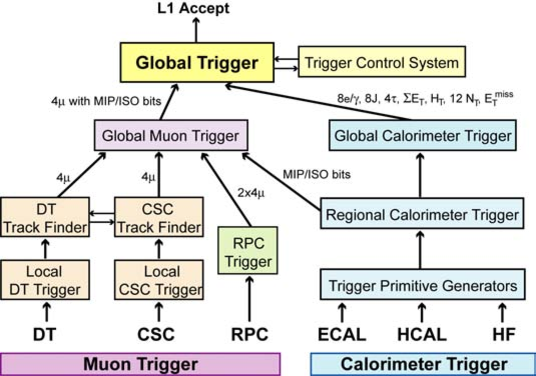
\includegraphics[width=0.7\textwidth]{fig/trigger}
\caption{The \ac{CMS} \acl{L1T}}
\label{fig:expt_cms_trigger}
\end{figure}

The structure of the \ac{L1T} is shown in Figure~\ref{fig:expt_cms_trigger}. At
the top sits the \ac{GT}. This receives objects from the two trigger subsystems:
the \ac{GCT} and \ac{GMT}. Objects are received, ranked according to their
energy and quality along with their coordinates in $\eta$ and $\phi$. These
objects are fed to 128 reprogrammable algorithms, each producing a trigger
decision. This trigger decision is then compared with a mask in order to give a
single decision. This mask may be altered as desired to achieve different
data-taking objectives. The final trigger decision is then sent to the Timing,
Trigger and Control subsystem in order to initiate a readout of the detector.

The calorimeter trigger subsystem begins with the \ac{TPG}. This sums energy
deposits from the \ac{ECAL} and \ac{HCAL} into trigger towers. This information
is received by the \ac{RCT}. This system is tasked with finding electron/photon
candidates and further summing the trigger tower energy measurements into
\ac{RCT} regions. These consist of $4\times 4$ trigger towers (except in the
\ac{HF} where only a single trigger tower is included). The \ac{RCT} also
records a ``tau-veto'' bit, used to distinguish jets from hadronic tau decays.

The output of the \ac{RCT} is then processed by the
\ac{GCT}~\cite{jj_thesis}. The \ac{GCT} logic is implemented entirely in
\acp{FPGA}. The \ac{GCT} has a number of responsibilities. Firstly, it sorts the
list of electron/photon candidates and passes the four highest ranked objects to
the \ac{GT}. Secondly, it performs a simple jet-finding algorithm on the energy
regions received from the \ac{RCT}. This identifies local maxima as jets and
distinguishes between \emph{forward}, \emph{central} and \emph{tau} jets. The
last category includes jets for which none of the constituent regions has the
aforementioned tau veto bit set. The four highest ranked of each category are
forwarded to the \ac{GCT}.

The final task of the \ac{GCT} is to form global energy sums. These are the
total transverse energy, missing transverse energy, jet counts and \HT (the
scalar sum of the jet energies). These too are forwarded to the \ac{GT} to be
used in the trigger decision.

The muon trigger receives input from all three muon subdetectors: \acp{RPC},
\acp{CSC} and \acp{DT}. These are integrated in the \ac{GMT} which also receives
isolation and minimum ionising particle information from the \ac{GCT} for each
calorimeter region. The muons received from each subdetector are matched and
sorted by transverse momentum and quality. The four highest rank candidates are
forwarded to the \ac{GT}.

\subsection{Computing at \ac{CMS}}
\label{sec:cms_computing}
To mee the extremely large computation and storage requirements of data analysis
at the \ac{LHC}, analysis tasks are performed using a dedicated computing
grid~\cite{lhc_grid}. Reconstructed events are sent to the ``tier-0'' storage
site at \ac{CERN} and additional copies are forwarded to a number of ``tier-1''
sites around the world. ``Tier-2'' and ``Tier-3'' sites make further copies of
data as required. User analysis jobs can then be submitted from any site and
routed to a site where the data is available.

Events recorded by the \ac{CMS} detector pass through a chain of reconstruction
stages. At each stage, higher-level physics objects are generally built out of
simpler ones, with a consequent reduction in the data size. Analysis users may
choose to perform their analysis on any of these layers, depending on their
needs. The processing and analysis tools make up the \cmssw software framework.

Monte Carlo events are processed using either a detailed \geantfour
simulation~\cite{geant_paper} or a faster, parameterised model of the response
known as \fastsim. This simulates the response of the \ac{CMS} subdetectors to
the generated particles, after which simulated and real data are processed
identically.
